%===================================================================================================
\subsection{HIV Progression \& Mortality}\label{mod.par.hiv}
%---------------------------------------------------------------------------------------------------
\subsubsection{HIV Progression}\label{mod.par.hiv.dur}
The length of time spent in each HIV stage is related to
rates of progression between stages $\eta_{h}$,
rates of additional HIV-attributable mortality by stage $\mu_{\textsc{hiv},h}$,
and treatment via antiretroviral therapy (ART).
\citet{Lodi2011} estimate median times from seroconversion to
\cdf{}{500}, $<$\,350, and $<$\,200 cells/mm\tsup{3}, while
\citet{Mangal2017} directly estimate the rates of progression between CD4 states $\eta_{h}$
in a simple compartmental model.
Based on these data, we modelled mean durations ($1/\eta_{h}$) of:%
\footnote{Assuming exponential distributions for durations in each CD4 state \cite{Roberts2015}.}
0.142 years in acute infection ($h=2$, from \sref{mod.par.beta.hiv});
3.35 years in \cdf{500}{} ($h=3$);
3.74 years in \cdf{350}{500} ($h=4$); and
5.26 years in \cdf{200}{350} ($h=5$); plus
the remaining time until death in \cdf{}{200} ($h=6$, AIDS).
Since the duration in acute infection ($h=2$) is randomly sampled,
the remaining duration in \cdf{500}{} ($h=3$) is adjusted accordingly.
%---------------------------------------------------------------------------------------------------
\subsubsection{HIV Mortality}\label{mod.par.hiv.mort}
Mortality rates by CD4-count in the absence of ART were estimated in
multiple African studies \cite{Badri2006,Anglaret2012,Mangal2017};
based on these data, we estimated yearly HIV-attributable mortality rates $\mu_{\textsc{hiv},h}$ as:
0 during acute phase ($h=2$);
0.4\% during \cdf{500}{} ($h=3$);
2\% during \cdf{350}{500} ($h=4$);
4\% during \cdf{200}{350} ($h=5$); and
20\% during \cdf{}{200} ($h=6$, AIDS).
%===================================================================================================
\subsection{Antiretroviral Therapy}\label{mod.par.art}
Viral suppression via antiretroviral therapy (ART) influences
the probability of HIV transmission, as well as rates of HIV progression and HIV-related mortality.
The model considers individuals on ART before ($c=3$) and after ($c=4$)
achieving full viral load suppression (VLS), as defined by undetectable HIV RNA in blood samples.
Among retained patients initiating ART (see \sref{mod.par.cascade.tx} for rates), time to VLS
is usually described as ``within 6 months'' \cite{Thompson2012}.
\citet{Mujugira2016} estimated the median time to VLS as 3.1 [IQR: 2.8,~5.5] months
from 1592 HIV serodiscordant couples;
however this time may be underestimated due to the trial conditions and population.
The distribution of time to VLS (Figure~1 in \cite{Mujugira2016}) also featured a heavy tail,
suggesting heterogeneity in time to VLS (see \sref{mod.par.cascade.dx} for implications).
For example, time to VLS may be prolonged due to social and economic barriers to care
\cite{Dlamini-Simelane2017,Horter2019}.
Considering these data, we sampled the time to VLS (duration in cascade state $c=3$)
from a gamma distribution with 95\%~CI (0.33,~1.0) years.
%---------------------------------------------------------------------------------------------------
\subsubsection{Probability of HIV Transmission on ART}\label{mod.par.art.beta}
All available evidence suggests that viral suppression by ART to undetectable levels
prevents HIV transmission, \ie undetectable = untransmittable (``U=U'') \cite{Eisinger2019uu}.
Thus, we assumed zero HIV transmission from individuals with VLS ($c=4$).
However, HIV transmission may still occur
during the period between ART initiation to viral suppression ($c=3$) \cite{Mujugira2016}.
\citet{Donnell2010} estimate an adjusted incidence ratio of 0.08~(0.0,~0.57) for all individuals on ART.
However, in \cite{Donnell2010} and \cite{Cohen2016}, the 1 and 4 (respectively)
genetically linked infections from individuals on ART all occurred within 90 days of ART initiation,
suggesting that risk of transmission only persists before viral suppression.
Adjusting the incidence denominator (person-time)
to 90 days per individual who initiated ART in \cite{Donnell2010}
results in approximately 3.13 times higher estimated incidence ratio: 0.25 for this specific period.%
\footnote{In \cite{Donnell2010}, individuals who initiated ART contributed
  approximately 9.4 months per-person (273 persons / 349 person-years, Tables~2~and~3);
  thus the first 3 months of each individual represent
  3/9.4 = 0.319 fewer person-months of follow-up.}
Thus, we sampled relative infectiousness on ART but before viral suppression ($c=3$)
from a BAB distribution with mean (95\%~CI) of 0.25~(0.01,~0.67).
Finally, we assumed that the virally un-suppressed state ($c=5$) had
half the reduced infectiousness of $c=3$, yielding 95\%~CI: (0.50,~0.83).
%---------------------------------------------------------------------------------------------------
\subsubsection{HIV Progression \& Mortality on ART}\label{mod.par.art.hiv}
\def\hunprog{$h = 6 \rightarrow 5 \rightarrow 4 \rightarrow 3$\xspace}
Effective ART stops CD4 cell decline and results in some CD4 recovery \cite{Battegay2006,Lawn2006}.
Most CD4 recovery occurs within the first year of treatment \cite{Battegay2006}.
Due to the limited number of modelled treatment states,
we model this initial recovery to be associated with the pre-VLS ART state ($c=3$).
\citet{Lawn2006,Gabillard2013} estimate an increase of between 25--39 cells/mm\tsup{3} per month
during the first 3 months of treatment.
After initial increases, CD4 recovery is modest and plateaus.
\citet{Battegay2006} report approximate increases of
22.4 cells/mm\tsup{3} per year between years 1 and 5 on ART.
Since HIV states $h=4,5,6$ correspond to 150, 150, and 200-wide CD4 strata,
we model rates of movement along \hunprog as
0.167, 0.167, 0.125 per month, respectively, during pre-VLS ART ($c=3$) and
0.1 per year after VLS ($c=4$).
\par
Since higher CD4 states are modelled to have lower mortality rates (see \sref{mod.par.hiv.mort}),
the modelled recovery of CD4 cells via ART described above implicitly affords a mortality benefit.
However, HIV infection is associated with increased risk of death by non-AIDS causes
--- \ie unrelated to CD4 count ---
including cardiovascular disease and renal disease \cite{Phillips2008}.
\citet{Lundgren2015init} estimated 61\% reduction in non-AIDS life-threatening events due to ART.
For the same CD4 strata, \citet{Gabillard2013} also report approximately 2-times higher
mortality rates within the first year of ART \vs thereafter,
suggesting that VLS is associated with 50\% mortality reduction independent of CD4 increase.
Thus, we modelled an additional 50\% reduction in mortality among individuals with VLS ($c=4$),
and half this (25\%) reduction before achieving VLS ($c=3$).
%===================================================================================================
\subsection{Rates of HIV Diagnosis, ART Initiation, Viral Un-suppression \& Re-suppression}\label{mod.par.cascade}
% TODO: (?) add Walsh2020
Rates of HIV diagnosis $\delta$, ART initiation $\tau$, viral un-suppression $\zeta$
(including treatment failure, discontinuation, or loss to follow-up),
and viral re-suppression $\sigma'$ (Figure~\ref{fig:model.cascade})
were defined to reflect historical trends and ART eligibility for Eswatini
\cite{EswMOH2006gui,EswMOH2010gui,EswMOH2015gui,EswMOH2018gui}, as described in detail below.
These rates were further calibrated to reproduce observed cascade attainment over time in Eswatini
(\eg proportion on ART among those diagnosed with HIV).
Similar to condom use, rates were interpolated between specified years
using monotone piecewise cubic interpolation \cite{Fritsch1980}.
%---------------------------------------------------------------------------------------------------
\subsubsection{HIV Diagnosis}\label{mod.par.cascade.dx}
Multiple Eswatini studies report the proportions of women and men who tested for HIV in the p12m.
However, this proportion may not directly reflect the yearly rate of diagnosis,
because individuals may test more frequently based on their perceived risk \cite{Witzel2017}.
Indeed, EmaSwati living with HIV were more likely to have reported previously testing for HIV in
2006 \cite[Table~14.9]{SDHS2006}, 2011 \cite[Table~5]{SHIMS1T}, and 2016 \cite[Table~7.3]{SHIMS2}.
Additionally, the proportion tested in p12m
likely underestimates the \emph{rate} of testing due to repeat testers.
Assuming an exponentially-distributed time spent untested in the period under consideration
(consistent with inherent compartmental modelling assumptions),
the testing rate $\lambda$ can be calculated
from the proportion tested $\rho$ over period $T$ via:
\begin{equation}\label{eq:exp.decay}
  \begin{aligned}
       \rho &= 1 - \exp{(-\lambda T)} \\
    \lambda &= - \log{(1-\rho)} / T
  \end{aligned}
\end{equation}
Moreover, \cite{Behanzin2013} found approximately 70\% underreporting of ever testing for HIV
in face-to-face interviews \vs anonymous polling booth surveys,
with consistent results across married and unmarried women and men.
\par
Yet, preliminary model calibration
using reported HIV testing rates (with 95\%~CI) described below as HIV diagnosis rates directly
caused the model to overestimate HIV+ status awareness \vs the available data
(see \sref{mod.cal.targ.cascade}, Table~\ref{tab:targ.cascade}).
This apparent discrepancy between reported population-level testing rates and HIV+ status awareness
is in fact common, and could be explained by testing rate heterogeneity \cite{Maheu-Giroux2019f90}
--- \ie the existance of ``fixed'' sub-populations
who test frequently and those who test rarely or never.
Without further stratifying the modelled population along this testing frequency dimension,
it is impossible to capture this heterogeneity directly.
However, an alternative solution is to reduce modelled HIV diagnosis rates
to reproduce the available data on HIV+ status awareness via model calibration.
To this end, we parameterized HIV diagnosis rates over time based on reported testing rates (below),
with a global reduction factor $f \sim \opname{Unif}(0.5,1)$.
We further specified diagnosis rates using non-FSW women as a reference group,
with separate time-varying \emph{relative} rates defined for FSW and men.
Confidence intervals for relative rates were assumed using
a standard deviation of 0.2 for FSW and 0.1 for men (gamma priors).
%---------------------------------------------------------------------------------------------------
\paragraph{HIV Testing Rates}
Early HIV testing in Eswatini was mainly available to pregnant women via antenatal clinics,
though a small number of youth and men also accessed HIV testing services \cite{EswHPC1998,HSRC2004}.
Based on antenatal clinic data \cite{EswUNGASS2010},
we modelled a gradual increase in rates of HIV diagnosis among women
from zero to 95\%~CI (5,~15)\% (gamma prior) per year from 1990 to 2002,
when the national HIV testing and counselling program was formally introduced \cite{NERCHA2012rep}.
We assumed no initial differences between FSW and other women,
due to the lack of specific key populations prevention programs \cite{EswNASA2006}.
We further assumed that HIV diagnosis among men initially occurred at 10\% the rate of women.
\par
By 2006, $\rho = {}$21.9~(20.6,~23.3)\% of women and 8.9~(7.8,~10.0)\% of men
had tested for HIV and received the results in p12m \cite{SDHS2006}%
\footnote{Unless otherwise noted, \shortquote{tested for HIV} will imply
  \shortquote{and received the results} throughout this section.}
--- relative rate for men \vs women: 0.377~(0.207,~0.597).
Further scale-up of HIV testing began in 2006 via provider-initiated testing
and improved integration with the general health care system \cite{NERCHA2012rep}.
Between 2007 and 2010, such efforts
doubled the number of testing locations (119 to 241) and
tripled the number of total yearly tests (53,000 to 154,000) \cite{NERCHA2009nsf,NERCHA2012rep}.
By 2011, an estimated $\rho = {}$46.8\% of women, 28.4\% of men, and 61.7~(55.6,~67.5)\% of FSW
had tested for HIV in p12m \cite{SHIMS1T,Baral2014},%
\footnote{The adjustment for missing ages 15--17 in \cite{SHIMS1T} from \sref{mod.cal.targ.prev}
  was applied to the reported 50.1\% of women and 31.7\% of men aged 18--49 who tested in p12m,
  assuming 20\% of women and 10\% of men aged 15--17 tested in p12m.}
yielding testing rates of $\lambda = {}$0.631, 0.333, and 0.962 per year, respectively
--- relative rates: 0.529~(0.352,~0.743) for men, and 1.521~(1.206,~1.980) for FSW.
\par
% TODO: (?) 2014 eNSF KP programs started
% TODO: (?) Testing Reasonably consistent across age groups \cite[Figure~7.3.A]{SHIMS2}
Phase~1 of the MaxART program \cite{MaxART1} ran from 2011 to 2014,
with a primary objective to increase HIV testing.
An estimated 284,680 people were reached with 389,658 tests by the end of Phase~1 (2014).
By 2016, 57.1\% of women and 47.8\% of men had tested in p12m \cite{SHIMS2},
yielding testing rates of $\lambda = {}$0.846 and 0.650 per year, respectively.
The relative rate for men increased to 0.770~(0.587,~0.978);
however, this increase was \emph{not} applied (2011 relative rate maintained)
to improve model fit (see \sref{mod.cal}).
In 2014 \cite{EswKP2014} and 2020 \cite{EswIBBS2022}
approximately $\rho = {}$75\% of FSW had tested in p12m ($\lambda = 1.386$)
as such, we applied a relative rate of 1.62,~(1.29,~2.07) for 2016.
We held all rates of HIV diagnosis after 2016 fixed.
%---------------------------------------------------------------------------------------------------
\subsubsection{ART Initiation}\label{mod.par.cascade.tx}
Rates of ART initiation $\tau$ were modelled to reflect
time-varying eligibility, availability, loss to follow-up,
and differences between sex/activity groups.
%---------------------------------------------------------------------------------------------------
\paragraph{Eligibility}
Historical ART eligibility in Eswatini has generally followed
the evolving World Health Organization (WHO) guidelines
\cite{WHO2003art,WHO2007art,WHO2013art,WHO2016art}.
Initial eligibility included one of \cite{EswMOH2006gui}:
\begin{itemize}
  \item \cdf{}{200} cells/mm\tsup{3} and any WHO clinical stage
  \item \cdf{}{350} cells/mm\tsup{3} and WHO clinical stage III
  \item any CD4 count and WHO clinical stage IV
\end{itemize}
Eligibility was revised in 2010 \cite{EswMOH2010gui} to:
\begin{itemize}
  \item \cdf{}{350} cells/mm\tsup{3} and any WHO clinical stage
  \item any CD4 count and WHO clinical stage III or IV
\end{itemize}
and again in 2015 \cite{EswMOH2015gui} to:
\begin{itemize}
  \item \cdf{}{500} cells/mm\tsup{3} and any WHO clinical stage
  \item in a discordant partnership or having a specified illness (any CD4 count or WHO clinical stage)
\end{itemize}
before adoption of the current \shortquote{ART for all} guidelines
in late 2016 (modelled as effectively January 2017) \cite{MaxART2,EswMOH2018gui}.
Phase~2 of MaxART also began in 2015, offering immediate ART
via 14 health facilities in a stepped wedge design (6 facilities added per year) \cite{MaxART2}.
Relative to the 114 total facilities offering ART nationally at this time \cite{NERCHA2014nsf},
we assumed this trial had minimal direct impact on population-level ART initiation
--- notwithstanding valuable insights gained regarding effective implementation \cite{MaxART2}.
\par
We implemented the CD4-only eligibility criteria directly in the model,
which is structured to match these 200, 350, and 500 CD4 cells/mm\tsup{3} thresholds
(Figure~\ref{fig:model.hiv}).
For eligibility by WHO clinical stages (not explicitly modelled),
we estimated relative rates of ART initiation based on the following data from
South Africa \cite[Table~4]{Badri2004} and Saudi Arabia \cite[Table~2]{Edathodu2009}, respectively:
\begin{itemize}
  \item 43/111~(39\%) and 14/46~(30\%) of PLHIV with \cdf{200}{350} were at stages III or IV;\\
        assumed: 35\% PLHIV with \cdf{200}{350} were eligible for ART pre-2010
  \item 13/79~(16\%) and 6/76~(8\%) of PLHIV with \cdf{350}{} were at stage III;\\
        assumed: 15\% PLHIV with \cdf{350}{500} were eligible for ART pre-2010
        (5\% with \cdf{500}{})
  \item 5/79~(6\%) and 1/76~(1\%) of PLHIV with \cdf{350}{} were at stage IV;\\
        assumed: 20\% PLHIV with \cdf{350}{500} were eligible for ART 2010--2015
        (5\% with \cdf{500}{})
\end{itemize}
We assumed that roll-out of eligibility changes in 2010, 2015, and 2017
each occurred over a 1-year period.
Figure~\ref{fig:art.elig} illustrates
the resulting modelled relative rates of ART initiation for each HIV stage over time.
\begin{figure}
  \centering
  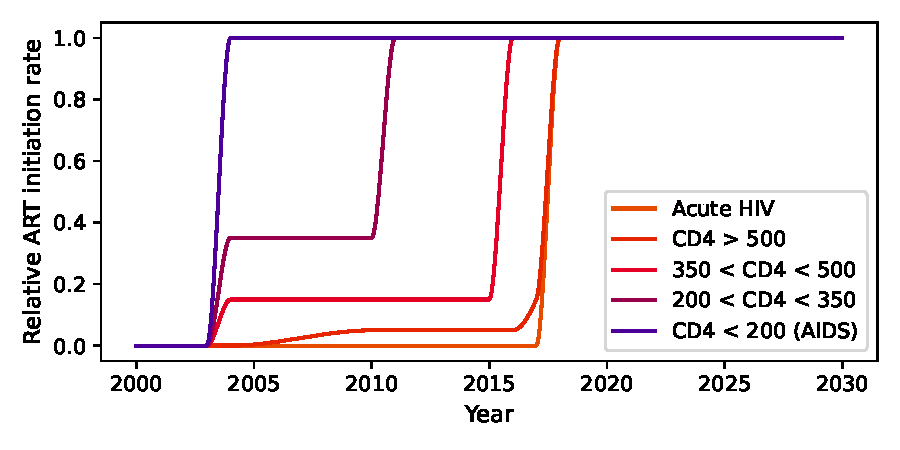
\includegraphics[scale=\fitscale]{art.elig}
  \caption{Modelled relative rates of ART initiation by HIV stage,
    reflecting eligibility changes over time}
  \label{fig:art.elig}
\end{figure}
%---------------------------------------------------------------------------------------------------
\paragraph{Availability and Initiation}
ART first became available in Eswatini in late 2003
via a one-hospital pilot project \cite{NERCHA2012rep}.
Early ART scale-up was modest, with 31 facilities offering ART by the end of 2009 \cite{CDC2013art};
however, this number increased rapidly
to 110 facilities by the end of 2011 \cite{NERCHA2012rep}.
Phase~1 of MaxART (2011--2014) sought to
further increase ART coverage among eligible PLHIV \cite{MaxART1},
including decentralization to lower level facilities,
bringing the total number of facilities to 170 by 2015 \cite{EswMOH2015rep}.
Finally, national adoption of \shortquote{Test and Start} in 2017
likely further reduced delays in ART initiation,
while loss to follow-up was reduced throughout the years of ART scale-up \cite{MaxART2}.
\par
Considering these data, we modelled the yearly ART initiation rate among eligible diagnosed PLHIV as:
effectively $\tau = 0$ in 2003, gradually increasing to 1.5~(0.5,~3.0) by 2010;
then to 9~(6,~12) by 2012; and stabilizing at 12 by 2018.
This maximum rate of $\tau = 12$ corresponds to
a mean effective delay of one month between diagnosis and ART initiation;
this value was chosen in part to avoid numerical instability
when solving the model with very high rates.
%---------------------------------------------------------------------------------------------------
\paragraph{Group Differences}
In 2011, conditional ART coverage (among diagnosed) was greater among men \vs women
(Table~\ref{tab:targ.cascade}),
suggesting greater ART initiation among men \vs women.
Yet, unconditional ART coverage (among PLHIV, regardless of diagnosis)
were approximately equal (31.4 and 33.2\%, respectively),
and so conditional differences may be explained by the fact that
women were more likely to be diagnosed at an earlier HIV stage via antenatal care,
and thereafter not yet eligible for ART.
Thus, we assumed no differences in ART initiation among men \vs women.
A similar mechanism could partially explain
differences in conditional coverage between FSW \vs women overall (36.9 \vs 48.0\%),
as FSW were more slightly likely to know their status (74.1 \vs 69.1\%).
However, FSW face unique barriers to accessing ART
related to stigma and material insecurity \cite{Lancaster2016sr};
as such, we sampled a relative rate for ART initiation among FSW from [0.5,~1] (uniform prior).
% TODO: (?) remove in later years?
%---------------------------------------------------------------------------------------------------
\subsubsection{ART Failure}\label{mod.par.cascade.fail}
% TODO: (~) add Jobanputra2015
The modelled virally un-suppressed state ($c=5$) reflects any combination of
treatment failure (\ie due to resistance mutations),
discontinuation, or loss to follow-up (LTFU) after achieving viral suppression.
The model does not explicitly simulate emergence and/or transmission of drug resistance,
nor multiple unique ART regimens.
As of 2016, resistance mutations to at least 1 of 3 drugs in combination regimens
were identified in 10\% ART-naive PLHIV in Eswatini,
and 16\% PLHIV with prior ART exposure \cite{WHO2021dr}.
However, the extent to which these individual mutations can cause
complete treatment failure remains unclear. % TODO: (~) SM or RK can help?
Additionally, while transmissible resistance mutations could become more prevalent over time,
emergence of new drugs can combat the population-level impacts of this resistance \cite{Hauser2019}.
\par
All available data suggests that retention in ART care
--- \ie not discontinued or LTFU ---
has improved over time in Eswatini \cite{NERCHA2014garp,NERCHA2018rep,SHIMS2}.
Assuming an exponentially-distributed retention time
(consistent with inherent compartmental modelling assumptions),
we averaged the available data \cite[Table~6]{NERCHA2018rep}
to calculated the effective yearly ART attrition rate as:
16.5\% in 2008, 13.8\% in 2010, 14.1\% in 2012, and 8.3\% in 2014.
One-year LTFU was reported as 1\% in 2016 \cite{SHIMS2},
but it's not clear whether this definition was consistent with the earlier estimates.
Many measures of LTFU may also overestimate true LTFU
by failing to account for transfers between clinics and deaths \cite{Fox2018,Wilkinson2015};
it's not clear whether the reported measures for Eswatini account for transfers or deaths.
\par
LTFU was estimated to be 1.3 times higher among men \vs women in South Africa \cite{Fox2018},
which would be consistent with observed lower viral suppression among men \vs women on ART
in Eswatini (Table~\ref{tab:targ.cascade}) \cite{Fox2018}.
The same study estimated that LTFU did not significantly differ
by the modelled CD4-strata \cite{Fox2018}.
No estimates of LTFU were available for FSW specifically in Eswatini,
but among 354 FSW on ART in \cite{EswIBBS2022} (2021),
103 knew the results of viral load monitoring in p12m,
of whom only 8 self-reported undetectable viral load.
Such data may again reflect the unique barriers to accessing ART faced by FSW \cite{Lancaster2016sr}.
\par
Considering all of the above data,  assumed:
a yearly rate of viral un-suppression $\zeta$ among non-FSW women of
15\% until 2010, decreasing to 5\% by 2018;
plus relative rates for men and FSW: [1,~1.5] (uniform priors).
%---------------------------------------------------------------------------------------------------
\subsubsection{Viral Re-suppression}\label{mod.par.cascade.retx}
The rate of viral re-suppression $\sigma'$ aims to reflect the average delay associated with
the steps of switching regimens (in case of treatment failure), or
the steps of re-engaging in HIV care (in case of LTFU).
\par
For treatment failure, viral un-suppression must first be identified.
Availability of viral load monitoring in Eswatini was limited until at least 2010 \cite{EswMOH2010gui},
but incorporated into standard of care by 2015 (yearly testing) \cite{EswMOH2015gui}.
Without viral load testing, treatment failure can still be indicated clinically \cite{EswMOH2010gui}.
After suspecting treatment failure,
at least three months of additional monitoring is typically required
to rule-out issues of adherence \cite{EswMOH2010gui,EswMOH2015gui,EswMOH2018gui},
before another regimen is started.
Moreover, second/third-line regimen options
were limited in Eswatini until at least 2014 \cite{Jobanputra2015,NERCHA2014nsf}.
Upon switching to an improved regimen,  assume that viral suppression occurs
at the same rate as among ART-naive PLHIV (see \sref{mod.par.art}).
\par
For LTFU, no data directly indicate the average duration out of care in Eswatini.
A recent model-based analysis of Kenyan data \cite{Bakoyannis2020} suggests
an average between 8 months and 2 years.
Considering large-scale, multisectorial efforts to improve ART care in Eswatini,
it is likely that duration out of care has declined since 2010.
Thus,  sampled the initial rate of viral re-suppression $\sigma'$ from
a gamma prior with 95\% [0.5,~1.0], which increased by a factor of 1.5 over 2010--2018.
We assumed no differences between groups.
